\section{Appendix: Governing Equations}

\setcounter{equation}{0}

\subsection{Mode: {\tt RICHARDS}}

{\tt RICHARDS} Mode applies to single phase, variably saturated, isothermal systems. The governing mass conservation equation is given by
\EQ
\frac{\p}{\p t}\left(\varphi s\rho\right) + \bnabla\cdot\left(\rho\bq\right) = Q_w,
\EN
with Darcy flux $\bq$ defined as
\EQ
\bq = -\frac{kk_r(s)}{\mu}\bnabla\left(P-W_w\rho g z\right).
\EN
Here, $\varphi$ denotes porosity [-], 
$s$ saturation [m$^3$m$^{-3}$], 
$\rho$ water density [kmol m$^{-3}$], 
$\bq$ Darcy flux [m s$^{-1}$], 
$k$ intrinsic permeability [m$^2$], 
$k_r$ relative permeability [-], 
$\mu$ viscosity [Pa s], 
$P$ pressure [Pa], 
$W_w$ formula weight of water [kg kmol$^{-1}$], 
$g$ gravity [m s$^{-2}$], and 
$z$ the vertical component of the position vector [m].  
Supported relative permeability functions $k_r$ for Richards' equation include van Genuchten, Books-Corey and Thomeer-Corey, while the saturation functions include Burdine and Mualem.  Water density and viscosity are computed as a function of temperature and pressure through an equation of state for water. The source/sink term $Q_w$ [kmol m$^{-3}$ s$^{-1}$] has the form
\EQ
Q_w \eq \frac{q_M}{W_w} \delta(\br-\br_{ss}),
\EN
where $q_M$ denotes a mass rate in kg/m$^{3}$/s, and $\br_{ss}$ denotes the location of the source/sink.

\subsection{Capillary Pressure Relations}

Capillary pressure is related to saturation by various 
phenomenological relations, one of which is the van Genuchten 
(1980) relation 
\EQ\label{seff}
s_e \eq \left[1+\left( \frac{p_c}{p_c^0} \right)^n 
\right]^{-m}, 
\EN 
where $p_c$ represents the capillary pressure [Pa], and the effective saturation $s_e$ is defined by 
\EQ 
s_e \eq \frac{s - s_r}{s_0 - s_r}, 
\EN 
where $s_r$ denotes the residual saturation, and $s_0$ denotes 
the maximum saturation. 
The inverse relation is given by
\EQ
p_c \eq p_c^0 \left(s_e^{-1/m}-1\right)^{1/n}.
\EN
The quantities $m$, $n$ and $p_c^0$ are impirical constants determined by fitting to experimental data.

\subsubsection{Brooks-Corey Saturation Function} 

The Brooks-Corey saturation function is a limiting form of the van Genuchten relation for $p_c/p_c^0 \gg 1$, with the form
\EQ
s_e \eq \left(\frac{p_c}{p_c^0}\right)^{-\lambda},
\EN
with $\lambda=mn$ and inverse relation
\EQ
p_c \eq p_c^0 s_e^{-1/\lambda}.
\EN

\subsubsection{Relative Permeability}

Two forms of the relative permeability function are implemented based on the Mualem and Burdine formulations.
The quantity $n$ is related to $m$ by 
the expression 
\EQ\label{lambda_mualem} 
m \eq 1-\frac{1}{n}, \ \ \ \ \ n \eq \frac{1}{1-m}, 
\EN 
for the Mualem formulation and by
\EQ\label{lambda_burdine} 
m \eq 1-\frac{2}{n}, \ \ \ \ \ n \eq \frac{2}{1-m}, 
\EN 
for the Burdine formulation.

For the Mualem relative permeability function based on the van Genuchten saturation function is given by the expression 
\EQ\label{krl_mualem} 
k_{r} \eq \sqrt{s_e} \left\{1 - \left[1- \left( s_e \right)^{1/m} \right]^m \right\}^2. 
\EN 
%and for the gas phase by 
%\EQ 
%k_{rg} \eq 1 - k_{rl}. 
%\EN 

The Mualem relative permeability function based on the Brooks-Corey saturation function is defined by 
\BA
k_r &\eq \big(s_e\big)^{5/2+2/\lambda},\\
&\eq \big(p_c/p_c^0\big)^{-(5\lambda/2+2)}.
\EA

For the Burdine relative permeability function based on the van Genuchten saturation function is given by the expression
\EQ\label{krl_burdine} 
k_{r} \eq s_e^2 \left\{1 - \left[1- \left( s_e \right)^{1/m} \right]^m \right\}. 
\EN 
The Burdine relative permeability function based on the Brooks-Corey saturation function has the form
\BA
k_r &\eq \big(s_e\big)^{2+3/\lambda},\\
&\eq \left(\frac{p_c}{p_c^0}\right)^{-(2+3\lambda)}.
\EA

\begin{comment}
\subsubsection{Linear} 
 
The linear relation is defined by 
\EQ\label{linear} 
k_{rl} \eq s_*, \ \ \ k_{rg} \eq 1-k_{rl}, \ \ \ s_* \eq \frac{s_l 
- s_l^r}{1-s_l^r}. 
\EN 
\end{comment}

\subsubsection{Smoothing}

At the end points of the saturation and relative permeability functions it is sometimes necessary to smooth the functions in order for the Newton-Raphson equations to converge. This is accomplished using a third order polynomial interpolation by matching the values of the function to be fit (capillary pressure or relative permeability), and imposing zero slope at the fully saturated end point and matching the derivative at a chosen variably saturated point that is close to fully saturated. The resulting equations for coefficients $a_i$, $i=0-3$, are given by
\begin{subequations}
\BA
a_0 + a_1 x_1 + a_2 x_1^2 + a_3 x_1^3 &\eq f_1,\\
a_0 + a_1 x_2 + a_2 x_2^2 + a_3 x_2^3 &\eq f_1,\\
a_1 x_1 + a_2 x_1^2 + a_3 x_1^3 &\eq f_1',\\
a_1 x_2 + a_2 x_2^2 + a_3 x_2^3 &\eq f_2',
\EA
\end{subequations}
for chosen points $x_1$ and $x_2$. In matrix form these equations become
\EQ
\begin{bmatrix}
1 & x_1 & x_1^2 & x_1^3\\
1 & x_2 & x_2^2 & x_2^3\\
0 & 1 & 2x_1 & 3x_1^2\\
0 & 1 & 2x_2 & 3x_2^2
\end{bmatrix}
\begin{bmatrix}
a_0\\
a_1\\
a_2\\
a_3
\end{bmatrix}
\eq
\begin{bmatrix}
f_1\\
f_2\\
f_1'\\
f_2'
\end{bmatrix}.
\EN
The conditions imposed on the smoothing equations for capillary pressure $f=s_e(p_c)$ are 
$x_1=2 p_c^0$, $x_2=p_c^0/2$, $f_1 = (s_e)_1$, $f_2 = 1$, $f_1' = (s_e')_1$, $f_2' = 0$.
For relative permeability $f=k_r(s_e)$, $x_1 = 1$, $x_2 = 0.99$, $f_1 = 1$, $f_2 = (k_r)_2$, $f_1' = 0$, $f_2' = (k_r')_2$. 

\begin{comment}
\subsection{Kelvin's Equations for Vapor Pressure Lowering} 
 
Vapor pressure lowering resulting from capillary suction is 
described by Kelvin's equation 
\EQ\label{vplwr} 
P_v \eq P_{\rm sat}(T) \e^{-P_c/n_l RT}, 
\EN 
where $P_v$ represents the vapor pressure, $P_{\rm sat}$ the 
saturation pressure of pure water, $T$ denotes the absolute 
temperature and $R$ denotes the gas constant. Note that the density 
of the liquid phase, $n_l$, is represented on a molar basis. 
\end{comment}

\subsection{Mode: {\tt MPHASE}}

Local equilibrium is assumed between phases for modeling multiphase systems with PFLOTRAN. The multiphase partial differential equations for mass and energy conservation solved by PFLOTRAN have the general form:
\begin{subequations}
\BA\label{mass_conservation_equation}
\frac{\p}{\p t} \bigg(\varphi \sum_\a s_\a^{}\eta_\a^{} x_i^\a \bigg)
+ \bnabla\cdot\sum_\a\bF_i^\a \eq Q_i,
\EA
for the $i$th component with flux $\bF_i^\a$
\EQ
\bF_i^\a \eq \bq_\a^{}\eta_\a^{} x_i^\a 
 - \varphi s_\a^{} D_\a^{} \eta_\a^{} \bnabla x_i^\a,
\EN
and
\BA\label{energy_equation}
\frac{\p}{\p t} \bigg(\varphi \sum_\a s_\a\eta_\a U_\a + (1-\varphi) \rho_r c_r T\bigg)
+ \bnabla\cdot\sum_\a\bigg[\bq_\a\eta_\a H_\a - \kappa\bnabla T\bigg] \eq Q_e.
\EA
\end{subequations}
for energy. 
In these equations $\a$ designates a fluid phase ($\a=\textrm{H}_\textrm{2}$O, supercritical CO$_\textrm{2}$) at temperature $T$ and pressure $P_\a$ with the sums over all fluid phases present in the system, and source/sink terms $Q_i$ and $Q_e$ described in more detail below. 
Species are designated by the subscript $i$ 
($i\!=\!\textrm{H}_\textrm{2}\textrm{O}$, $\textrm{CO}_\textrm{2}$); 
$\varphi$ denotes the porosity of the porous medium; 
$s_\a$ denotes the phase saturation state; 
$x_i^\a$ denotes the mole fraction of species $i$ ($\sum_i x_i^\alpha=1$); 
$\eta_\a$, $H_\a$, $U_\a$ refer to the molar density, enthalpy, and internal energy of each fluid phase, respectively; and 
$\bq_\a$ denotes the Darcy flow rate for phase $\a$ defined by
\EQ
\bq_\a \eq -\frac{kk_\a}{\mu_\a} \bnabla \big(P_\a-\rho_\a g \bz\big),
\EN
where $k$ refers to the intrinsic permeability, $k_\a$ denotes the relative permeability, $\mu_\a$ denotes the fluid viscosity, $W_\a^{}$ denotes the formula weight, $g$ denotes the acceleration of gravity, and $z$ designates the vertical of the position vector. The mass density $\rho_\a$ is related to the molar density by the expression
\EQ
\rho_\a = W_\a \eta_\a, 
\EN
where the formula weight $W_\a$ is a function of composition according to the relation
\EQ
W_\a \eq \frac{\rho_\a}{\eta_\a} \eq \sum_i W_i^{} x_i^\a.
\EN
The quantities $\rho_r$, $c_r$, and $\kappa$ refer to the mass density, heat capacity, and thermal conductivity of the porous rock. 

\subsubsection{Source/Sink Terms}

The source/sink terms, $Q_i$ and $Q_e$, describe injection and extraction of mass and heat, respectively, for various well models. Several different well models are available. The simplest is a volume or mass rate injection/production well given by
\begin{subequations}
\BA
Q_i &\eq \sum_n\sum_\a q_\a^V \eta_\a x_i^\a \delta(\br-\br_{n}),\\
&\eq \sum_n\sum_\a \frac{\eta_\a}{\rho_\a} q_\a^M x_i^\a \delta(\br-\br_{n}),\\
&\eq \sum_n\sum_\a W_\a^{-1} q_\a^M x_i^\a \delta(\br-\br_{n}),
\EA
\end{subequations}
where $q_\a^V$, $q_\a^M$ refer to volume and mass rates with units m$^3$/s, kg/s, respectively, related by the density
\EQ
q_\a^M \eq \rho_\a q_\a^V.
\EN
The position vector $\br_{n}$ refers to the location of the $n$th source/sink.

A less simplistic approach is to specify the bottom well pressure to regulate the flow rate in the well. In this approach the mass flow rate is determined from the expression
\EQ
q_\a^M \eq \Gamma \rho_\a \frac{k_\a}{\mu_\a} \big(p_\a-p_\a^{\rm bw}\big),
\EN
with bottom well pressure $p_\a^{\rm bw}$, and where $\Gamma$ denotes the well factor (production index) given by
\EQ
\Gamma \eq \frac{2\pi k \Delta z}{\ln\big(r_e/r_w\big) +  \sigma -1/2}.
\EN
In this expression $k$ denotes the permeability of the porous medium, $\Delta z$ refers to the layer thickness, $r_e$ denotes the grid block radius, $r_w$ denotes the well radius, and $\sigma$ refers to the skin thickness factor. For a rectangular grid block of area $A=\Delta x \Delta y$, $r_e$ can be obtained from the relation
\EQ
r_e \eq \sqrt{A/\pi}.
\EN
See Peaceman (1977) and Coats and Ramesh (1982) for more details.

\subsubsection{Variable Switching}

In PFLOTRAN a variable switching approach is used to account for phase changes enforcing local equilibrium. According to the Gibbs phase rule there are a total of $N_C\!+\!1$ degrees of freedom where $N_C$ denotes the number of independent components. This can be seen by noting that the
intensive
degrees of freedom are equal to $N_{\rm int}\!=\!N_C \!-\! N_P \!+\!2$, where $N_P$ denotes the number of phases. The 
extensive
degrees of freedom equals $N_{\rm ext}\!=\!N_P\!-\!1.$ This gives a total number of degrees of freedom $N_{\rm dof}\!=\!N_{\rm int}\!+\!N_{\rm ext}\!=\!N_C\!+\!1$, independent of the number of phases $N_P$ in the system.
Primary variables for liquid, gas and two-phase systems are listed in Table~\ref{tvar}.
The conditions for phase changes to occur are considered in detail below.

\begin{table}\centering
\caption{Choice of primary variables.}\label{tvar}

\vspace{3mm}

\begin{tabular}{lccc}
\toprule
State & $X_1$ & $X_2$ & $X_3$\\
\midrule
liquid & $p_l$ & $T$ & $x_\c^l$\\
gas & $p_g$ & $T$ & $x_\c^g$\\
two-phase & $p_g$ & $T$ & $s_g$\\
\bottomrule
\end{tabular}
\end{table}


\paragraph{Gas: $(p_g,\,T,\,x_\c^g)$ $\rightarrow$ Two-Phase: $(p_g,\,T,\,s_g^{})$} ~

$\bullet$ gas $\rightarrow$ 2-ph: $x_\c^g \leq 1-\dfrac{P_{\rm sat}(T)}{p_g}$, \ or equivalently: $x_\w^g \geq \dfrac{P_{\rm sat}(T)}{p_g}$

\paragraph{Liquid: $(p_l,\,T,\,x_\c^l)$ $\rightarrow$ Two-phase: $(p_g,\,T,\,s_g^{})$} ~

$\bullet$ liq $\rightarrow$ 2-ph: $x_\c^l \geq x_\c^{eq}$

\noindent
The equilibrium mole fraction $x_\c^{eq}$ is given by
\EQ
x_\c^{eq} \eq \frac{m_\c}{W_\w^{-1} + m_\c +  \sum_{l\ne \w,\,\c} m_l},
\EN
where the molality at equilibrium is given by
\EQ
m_\c^{eq} \eq \left(1-\dfrac{P_{\rm sat}(T)}{p}\right)\frac{\phi_c p}{K_\c \gamma_\c},
\EN
where it is assumed that 
\EQ
y_\c^{} \eq 1-\dfrac{P_{\rm sat}(T)}{p}.
\EN

\paragraph{Two-Phase: $(p_g,\,T,\,s_g)$ $\rightarrow$ Liquid $(p_l,\,T,\,x_\c^l)$ or Gas $(p_g,\,T,\,x_\c^g)$} ~

Equilibrium in a two-phase $\w$--$\c$ system is defined as the equality of chemical potentials between the two phases as expressed by the relation
\EQ
f_\c^{} \eq y_\c^{}\phi_\c^{} p_g^{} \eq K_\c^{} \big(\gamma_\c^{} m_\c^{}\big),
\EN
where
\EQ
y_\c^{} \eq x_\c^g, \ \ \ \ x_\c^{} \eq x_\c^l,
\EN
\EQ
x_\w^g \eq \frac{P_{\rm sat}(T)}{p_g},
\EN
\EQ
y_\c^{} \eq 1-x_\w^g \eq 1-\frac{P_{\rm sat}(T)}{p_g},
\EN
From these equations a Henry coefficient-like relation can be written as
\EQ
y_\c^{} \eq \widetilde K_\c^{} x_\c^{},
\EN
where
\EQ
\widetilde K_\c^{} \eq\frac{\gamma_\c^{} K_\c^{}}{\phi_\c^{} p_g}\frac{m_\c}{x_\c}.
\EN

\noindent
$\bullet$ A phase change to single liquid or gas phase occurs if $s_g \leq 0$ or $s_g\geq 1$, respectively.

Conversion relations between mole fraction $(x_i)$, mass fraction $(w_i)$ and molality $(m_i)$ are as follows:

\noindent
Molality--mole fraction:
\EQ
m_i \eq \frac{n_i}{M_\w} \eq \frac{n_i}{W_\w n_\w} \eq \frac{x_i}{W_\w x_\w} \eq \frac{x_i}{W_\w \big(1-\sum_{l\ne\w} x_l\big)}
\EN
Mole fraction--molality:
\EQ
x_i \eq \frac{n_i}{N} \eq \frac{n_i}{M_\w}\frac{M_\w}{N} \eq \frac{m_i}{\sum m_l} \eq \frac{W_\w m_i}{1+W_\w\sum_{l\ne\w} m_l}
\EN
Mole fraction--mass fraction:
\EQ
x_i \eq \frac{n_i}{N} \eq \frac{W_i^{-1} W_i n_i}{\sum W_l^{-1} W_l n_l} \eq \frac{W_i^{-1} w_i}{\sum W_l^{-1} w_l}
\EN
Mass fraction--mole fraction:
\EQ
w_i \eq \frac{M_i}{M} \eq \frac{W_i n_i}{\sum W_l n_l} \eq \frac{W_i x_i}{\sum W_l x_l}
\EN

\subsection{Mode: {\tt IMMIS}}

The {\tt IMMIS} mode applies to multiple completely immiscible phases.
The code PIMS, parallel immiscible multiphase flow simulator, is a simplified version of the  MPHASE mode in which the dependency on thermodynamic relations have been removed, since for immiscible systems the solubility is identically zero for each component. In this case the number of components is equal to the number of phases, or degrees of freedom associated with each node for an isothermal system. The immiscible property removes the variable switching strategy used in MPHASE, which may be the most numerically difficult part of PFLOTRAN, and may cause problems for multi-level solvers. 
%The code PMIS, parallel miscible single phase flow, applies to a completely miscible multicomponent single phase system.

The governing equations solved by PIMS are given by
\EQ\label{mass}
\frac{\p}{\p t}\big(\varphi\rho_\a^{} s_\a^{}\big) + \bnabla\cdot \big(\rho_\a^{} \bq_\a \big) \eq Q_\a,
\EN
where the subscript $\a$ denotes an immiscible phase.
\begin{comment}
, and for PMIS
\EQ\label{massmis}
\frac{\p}{\p t}\big(\varphi\rho x_i^{}\big) + \bnabla\cdot \big(\rho \bq x_i \big) \eq Q_i,
\EN
for the $i$th component in a single phase system.
\end{comment}
In this equation $\varphi$ is porosity, $s_\a$, $\rho_\a$ refer to the $\a$th phase saturation and density, respectively, $\bq_\a$ is the Darcy velocity of the $\a$th phase given by
\EQ
\bq_\a \eq -\frac{kk_\a}{\mu_\a} \big(\bnabla p-\rho_\a g \hat\bz\big), 
\EN
with permeability $k$, relative permeability $k_\a$, fluid viscosity $\mu_\a$, and $Q_\a$ is the source/sink term.  
The selection of primary variables are pressure $p$ and $n\!-\!1$ independent phase saturation variables $s_\a, \a=1,...,n\!-\!1$ with
\EQ
\sum_{\a=1}^n s_\a = 1.
\EN
The mass conservation equations are coupled to the energy balance equation given by
\EQ
\frac{\p}{\p t} \Big(\varphi\sum_\a s_\a\rho_\a U_\a + (1-\varphi) \rho_r C_r T\Big) + \bnabla\cdot\Big(\sum_\a\rho_\a\bq_\a H_\a - \kappa\bnabla T\Big) \eq Q_e,
\EN
where $U_\a$, $H_\a$ denote the internal energy and enthalpy of the $\a$th fluid phase, $\kappa$ denotes the thermal conductivity of the bulk porous medium, $\rho_r$, $C_r$ denote the rock density and heat capacity, and $T$ refers to the temperature.
%, if incompressibility of all phases or one of them is assumed. In this case, the reference pressure has to be specified as a boundary condition.
%The primary variables also could be $s_i, i=1,...,n$, if suitable EOS are applied to every phases. Then the second type BC could be assigned to all boundaries.
Thus the number of equations is equal to number of phases plus one, which is equal to the number of unknowns: ($p$, $T$, $s_1$, \ldots, $s_{n-1}$).

\subsection{Mode: {\tt MISCIBLE}}

The miscible mode applies to a mixture of water and proplyene glycol (PPG). In terms of molar density for the mixture $\eta$ and mole fractions $x_i$, $i$=1 (water), $i$=2 (PPG), the mass conservation equations have the form
\EQ
\frac{\p}{\p t} \varphi \eta x_i + \bnabla\cdot\left[\bq\eta x_i - \varphi D \eta \bnabla x_i\right] \eq Q_i,
\EN
with source/sink term $Q_i$. It should be noted that the mass- and mole-fraction formulations of the conservation equations are not exactly equivalent. This is due to the diffusion term which gives an extra term when transformed from the mole-fraction to mass-fraction gradient.

The molar density $\eta$ is related to the mass density by
\EQ
\eta \eq W^{-1} \rho,
\EN
and
\EQ
W_i\eta x_i \eq \rho y_i.
\EN
It follows that
\EQ
W_i \eta \bnabla x_i \eq \rho \bnabla y_i + \rho y_i \bnabla \ln W.
\EN
The second term on the right-hand side is ignored.

Simple equations of state are provided for density [g/cm$^3$], viscosity [Pa s], and diffusivity [m$^2$/s]. The density is a function of both composition are pressrue with the form
\BA
\rho(y_1,\,p) &\eq \rho(y_1,\,p_0) + \left.\frac{\p\rho}{\p p}\right|_{p=p_0} (p-p_0),\\
&\eq  \rho(y_1,\,p_0) \big(1+\beta (p-p_0)\big),
\EA
with the compressibility $\beta(y_1)$ given by
\BA
\beta &\eq \left.\frac{1}{\rho}\frac{\p\rho}{\p p}\right|_{p=p_0},\\
&\eq 4.49758\times 10^{-10} y_1 + 5\times 10^{-10}(1-y_1),
\EA
and the mixture density at the reference pressure $p_0$ taken as atmospheric pressure is given by
\EQ
\rho(y_1,\,p_0) \eq \Big(\big((0.0806 y_1 - 0.203) y_1 + 0.0873\big) y_1 + 1.0341\Big)10^3,
\EN
with mass fraction of water $y_1$. 
The viscosity and diffusivity have the forms
\EQ
\mu(y_1) \eq 10^{\big(1.6743 (1-y_1) - 0.0758\big)} 10^{-3},
\EN
and
\EQ
D(y_1) \eq \Big(\big(((-4.021 y_1 + 9.1181) y_1 - 5.9703) y_1 
     + 0.4043\big) y_1 + 0.5687\Big) 10^{-9},
\EN
The mass fraction is related to mole fraction according to
\EQ
y_1 = \frac{x_1 W_{\rm H_2O}}{W},
\EN
where the mean formula weight $W$ is given by
\EQ
W = x_1 W_{\rm H_2O} + x_2 W_{\rm PPG},
\EN
with formula weights for water and proplyene glycol equal to $W_{\rm H_2O}$ = 18.01534 and $W_{\rm PPG}$ = 76.09 [kg/kmol].

Global mass conservation satisfies the relation
\EQ
\frac{d}{dt}M_i \eq -\int\bF_i\cdot\bdS + \int Q_i dV,
\EN
with
\EQ
M_i \eq \int \varphi \eta x_i dV.
\EN
In terms of mass fractions and mass density
\EQ
M_i^m \eq W_i M_i \eq \int \varphi \rho y_i dV.
\EN

\subsection{Mode: {\tt Air-Water}}

The {\tt Air-Water} mode involves two phase liquid water-gas flow coupled to the reactive transport mode. Mass conservation equations have the form
\EQ
\frac{\p}{\p t} \varphi \Big(s_l^{} \rho_l^{} x_i^l + s_g^{} \rho_g^{} x_i^g \Big) + \bnabla\cdot\Big(\bq_l^{} \rho_l^{} x_i^l + \bq_g \rho_g^{} x_i^g -\varphi s_l^{} D_l^{} \rho_l^{} \bnabla x_i^l -\varphi s_g^{} D_g^{} \rho_g^{} \bnabla x_i^g \Big) \eq Q_i^{},
\EN
for liquid and gas saturation $s_{l,\,g}^{}$, density $\rho_{l,\,g}^{}$, diffusivity $D_{l,\,g}^{}$, Darcy velocity $\bq_{l,\,g}^{}$ and mole fraction $x_i^{l,\,g}$.
The energy conservation equation can be written in the form
\EQ
\sum_{\a=l,\,g}\left\{\frac{\p}{\p t} \big(\varphi s_\a \rho_\a U_\a\big) + \bnabla\cdot\big(\bq_\a \rho_\a H_\a\big) \right\} + \frac{\p}{\p t} \Big((1-\varphi)\rho_r C_p T \big) - \bnabla\cdot (\kappa\bnabla T)\Big) \eq Q,
\EN
as the sum of contributions from liquid and gas fluid phases and rock,
with internal energy $U_\a$ and enthalpy $H_\a$ of fluid phase $\a$, rock heat capacity $C_p$ and thermal conductivity $\kappa$. Note that
\EQ
U_\a \eq H_\a -\frac{P_\a}{\rho_\a}.
\EN

 
Thermal conductivity $\kappa$ is determined from the equation (Somerton et 
al., 1974)  
\EQ\label{cond} 
\kappa \eq \kappa_{\rm dry} + \sqrt{s_l^{}} (\kappa_{\rm sat} - \kappa_{\rm dry}), 
\EN 
where $\kappa_{\rm dry}$ and $\kappa_{\rm sat}$ are dry and fully saturated rock thermal conductivities. 


\subsection{Mode: {\tt THC} (Thermal-Hydrologic-Chemical)}

The current implementation of the {\tt THC} mode applies only to mass and energy conservation equations and a single tracer ($i=1$ in Eqn.\eqref{thc} below) which are solved fully coupled. The conservation equation for the tracer is coupled to the mass and energy equations through the Darcy velocity $\bq$, saturation $s$, temperature $T$ and pressure $P$. However, for fluid density only a function of $T$ and $P$, the mass and energy conservation equations are not coupled to the tracer equation and, therefore, they could be solved independently from the tracer equation although this is not done in the {\tt THC} mode. Future generalizations of the {\tt THC} mode will include multicomponent variable density fluids.
In the current implementation the THC equations may be coupled to the reactive transport mode (see Section \ref{sec:chem}).

{\tt THC} mode applies to single phase, variably saturated, nonisothermal systems
with incorporation of density variations coupled to fluid flow. 
The governing equations for mass and energy are given by
\EQ\label{masseqn}
\frac{\p}{\p t}\left(\varphi s\rho\right) + \bnabla\cdot\left(\rho\bq\right) = Q_w,
\EN
and
\EQ
\frac{\p}{\p t}\big(\varphi s\rho U + (1-\varphi) \rho_p c_p T\big) + \bnabla\cdot\big(\rho\bq H -\kappa \bnabla T\big) = Q_e,
\EN
coupled to nonreactive solute transport equations representing e.g. NaCl with the form
\EQ\label{thc}
\frac{\p}{\p t} \varphi s \rho x_i + \bnabla\cdot\big(\bq \rho x_i -\varphi D \rho\bnabla x_i\big) \eq Q_i,
\EN
with mole fraction $x_i$, source term $Q_i$, and diffusion/dispersion coefficient $D$. 
In these equations the Darcy flow velocity $\bq$ is given by
\EQ
\bq = -\frac{kk_r}{\mu}\bnabla\left(P-W\rho g z\right).
\EN
Here, $\varphi$ denotes porosity, $s$ saturation, $\rho$ mixture density of the brine, $\bq$ Darcy flux, $k$ intrinsic permeability, $k_r$ relative permeability, $\mu$ viscosity, $P$ pressure, $g$ gravity, and $z$ the vertical component of the position vector.  Supported relative permeability functions $k_r$ for Richards' equation include van Genuchten, Books-Corey and Thomeer-Corey, while the saturation functions include Burdine and Mualem.  Water density and viscosity are computed as a function of temperature and pressure through an equation of state for water. The quantities  $\rho_p$, $c_p$, and $\kappa$ denotes the  density, heat capacity, and thermal conductivity of the porous medium-fluid system. The internal energy and enthalpy of the fluid, $U$ and $H$, are obtained from an equation of state for pure water. These two quantities are related by the thermodynamic expression
\EQ
U \eq H -\frac{P}{\rho}.
\EN
The mean formula weight $W$ is related to the fluid composition by
\EQ
W \eq \sum_i W_i x_i.
\EN
Summing this equation over all components $i$ using $\sum_ix_i=1$, leads to Eqn.\eqref{masseqn} with
\EQ
Q_w \eq \sum_i Q_i.
\EN
Additional constitutive relations are needed to close the set of governing equations.
 
%\subsubsection{Thermal Conductivity} 
 
Thermal conductivity is determined from the equation (Somerton et al., 1974)  
\EQ\label{cond1} 
\kappa \eq \kappa_{\rm dry} + \sqrt{s_l^{}} (\kappa_{\rm sat} - \kappa_{\rm dry}), 
\EN 
where $\kappa_{\rm dry}$ and $\kappa_{\rm sat}$ are dry and fully saturated rock thermal conductivities. 

\subsubsection{Modeling with ice}
In PFLOTRAN, to model with ice and water vapor, one must compile with the option \texttt{ice=1}. The formulation used involves solving a modified Richard's equation coupled with energy balance equation (in \texttt{THC} mode, the tracer transport equation is also solved). This formulation is different from Painter 2011, where a multiphase approach was used and mass balance for air was also solved for. In this formulation, we do not track the movement of air, and hence we do not consider the mass balance for air. The balance of mass and energy for the water component that can be in three phases (liquid, gas, ice) are given by
\SEQ
\BA
& \pfx{}{t}\left[ \phi \left( s_l \eta_l X_w^l + s_g \eta_g X_w^g + s_i \eta_i X_w^i \right) \right] + \boldsymbol{\nabla} \cdot \left[X_w^l \boldsymbol{v}_l \eta_l + X_w^g \eta_g \boldsymbol{v}_g \right] - \boldsymbol{\nabla} \cdot \left[\phi s_g \tau_g  \eta_g D_g \boldsymbol{\nabla} X^g_w \right] = Q_w, \\
& \pfx{}{t}\left[ \phi \left( s_l \eta_l U_l + s_g \eta_g U_g + s_i \eta_i U_i \right) + (1- \phi) \rho_r c_r T \right] + \boldsymbol{\nabla} \cdot \left[ \boldsymbol{v}_l \eta_l  H_l+   \boldsymbol{v}_g \eta_gH_g \right] - \boldsymbol{\nabla} \cdot \left[ \kappa \boldsymbol{\nabla} T\right] = Q_e,
\EA \label{eq:balance_eqns}
\SEN where the subscripts $l$, $i$, $g$ denote the liquid, ice and gas phases respectivley; $\phi$ is the porosity; $s_{\alpha}  (\alpha = i, l, g)$, is the saturation of the $\alpha$-th phase; $\eta_{\alpha} (\alpha = i, l, g)$ is the molar density of the $\alpha$-th phase; $\rho_g$, $\rho_l$ are the mass densities of the gas and liquid phases; $Q_w$ is the mass source of H$_2$O;  $X_w^{\alpha} (\alpha = i, l, g)$ is the mole fraction of H$_2$O in the $\alpha$-th phase;   $\tau_g$ is the tortuosity of the gas phase; $D_g$ is the diffusion coefficity in the gas phase;  $T$ is the temperature (assuming all the phases and the rock are in thermal equilibrium); $c_r$ is the specific heat of the rock; $\rho_r$ is the density of the rock; $U_{\alpha} (\alpha = i, l, g)$ is the molar internal energy of the $\alpha$-th phase; $H_{\alpha} (\alpha = l, g)$ is the molar enthalpy of the $\alpha$-the phase; $Q_e$ is the heat source; $\boldsymbol{\nabla}\, (\, )$ is the gradient operator; $\boldsymbol{\nabla}\cdot (\,)$ is the divergence operator. 

The Darcy velocity for the gas and liquid phases given as follows:
\SEQ
\BA
& \boldsymbol{v}_g = - \frac{k_{rg}k}{\mu_g} \boldsymbol{\nabla}\left[p_g - \rho_g g  z \right], \\
& \boldsymbol{v}_l = - \frac{k_{rl}k}{\mu_l} \boldsymbol{\nabla}\left[p_l - \rho_l g z \right], 
\EA
\label{eq:darcy}
\SEN 
\noindent where $k$ is the absolute permeability; $k_{r \alpha} (\alpha =  l, g)$ is the relative permeability of the $\alpha$-th phase; $\mu_{\alpha}  (\alpha =  l, g)$ is the viscosity of the $\alpha$-th phase; $p_{\alpha}  (\alpha =  l, g)$ is the partial pressure of the $\alpha$-th phase; $g$ is acceleration due to gravity, $z$ is the vertical distance from a reference datum;

Constraint on the saturations of the various phases of water are given by
\BA
& s_l + s_g + s_i = 1.
\EA
Furthermore, neglecting the amount of air in liquid and ice phases, we have
\BA
X_a^l = 0, X_a^i = 0 \Rightarrow X_w^l = 1, X_w^i =1,
\EA
and so Eqns.~\eqref{eq:balance_eqns},~\eqref{eq:darcy}, based on the assumption that $p_g$ is hydrostatic (i.e., $p_g = (p_g)_0 + \rho_g g z $),  reduce to
\SEQ
\label{eq:gov}
\BA
 &\pfx{}{t}\left[ \phi \left( s_g \eta_g X_w^g +s_l \eta_l + s_i \eta_i \right) \right] + \boldsymbol{\nabla} \cdot \left[\boldsymbol{v}_l \eta_l \right] - \boldsymbol{\nabla} \cdot \left[\phi s_g \tau_g  \eta_g D_g \boldsymbol{\nabla} X^g_w \right] = Q_w, \label{eq:gov1}\\
& \pfx{}{t}\left[ \phi \left( s_l \eta_l U_l + s_g \eta_g U_g + s_i \eta_i U_i \right) + (1- \phi) \rho_r c_r T \right] + \boldsymbol{\nabla} \cdot \left[ \boldsymbol{v}_l \eta_l  H_l \right] - \boldsymbol{\nabla} \cdot \left[ \kappa \boldsymbol{\nabla} T\right] = Q_e, \\
& \boldsymbol{v}_l = - \frac{k_{rl}k}{\mu_l} \boldsymbol{\nabla}\left[p_l - \rho_l g z \right]. \label{eq:gov2}
\EA
\SEN
In the above formulation, temperature and liquid pressure are chosen to be primary variables. We also ensure that complete dry-out doesn't occur, and that liquid is present at all times. With this approach, one doesn't have to change the primary variables based on the phases present.

In additon to the previously described balance equations, additional constitutive relations are required to model non-isothermal, multiphase flow of water. Assuming thermal equilibrium among the ice, liquid and vapor phases, the mole fraction of water in vapor phase is given by the relation,
\BA
& X_w^g = \frac{p_v}{p_g},
\EA
where $p_v$ is the vapor pressure, $p_g$ is the gas pressure (For our calculations we shall assume that $p_g$ = 1 atm throughout the domain). Vapor pressure is calculated using Kelvin's relation 
%(\cite{Edlefsen:193uq}) 
which includes vapor pressure lowering due to capillary effect as follows
\BA
p_v = P_{\text{sat}}(T) \text{exp}\left[\frac{P_{cgl}}{\eta_l R (T + 273.15)} \right],
\EA
where $P_{\text{sat}}$ is the saturated vapor pressure, $P_{cgl}$ is the liquid-gas capillary pressure, $R$ is the ideal gas constant. Empirical relations for saturated vapor pressure are used for both above and below freezing conditions. $\eta_g$ is calculated using ideal gas law.

To calculate the partition of ice, liquid and vapor phases, at a known temperature and liquid pressure, the following two relations are used (see Painter 2011):
\SEQ
\label{sats}
\BA
\frac{s_l}{s_l + s_g} = S_{*}\left(P_{cgl}\right), \label{sats1}\\
\frac{s_l}{s_l + s_i}  = S_{*}\left[\frac{\sigma_{gl}}{\sigma_{il}} P_{cil} \right], \label{sats2}
\EA
\SEN
$S_{*}$ is the retention curve for unfrozen liquid-gas phases, $P_{cgl}$ is the gas-liquid capillary pressure, $P_{cil}$ is the ice-liquid capillary pressure, $\sigma_{il}$ and $\sigma_{gl}$ are the ice-liquid and gas-liquid interfacial tensions. Also, $P_{cil} = -\rho_i h_{iw} \vartheta $, where $h_{iw}^0$ is the heat of fusion of ice at 273.15 K, $\rho_i$ is the mass density of ice, $\vartheta = \frac{T - T_0}{T_0}$ with $T_0 = 273.15$ K.


For $S_{*}$, we use van Genuchten's model % (\cite{Genuchten1980A-closed-form-e}),
as follows:
\BA
S_{*} = \begin{cases}
           \left[ 1 + \left(\alpha {P_c}\right)^\gamma\right]^{-\lambda} , &\quad P_c > 0\\
           1, &\quad P_c \leq 0
            \end{cases}
\EA
with Mualem model % (\cite{Mualem1976A-new-model-for}) 
for the relative permeability of liquid water,
\BA
k_{rl} = (s_l)^{\frac{1}{2}} \left[1 - \left( 1 - (s_l)^{\frac{1}{\lambda}}\right)^{\lambda} \right]^2,
\EA
where $\lambda$, $\alpha$ are parameters, with $\gamma =  \frac{1}{1-\lambda}$.

The thermal conductivity for the frozen soil is chosen to be 
\BA
\kappa = Ke_{f} \kappa_{\text{wet},f} + Ke_{u} \kappa_{\text{wet},u} + (1 - Ke_u - Ke_f) \kappa_{\text{dry}},
\EA
where $\kappa_{\text{wet},f}$, $\kappa_{\text{wet},u}$ are the liquid- and ice-saturated thermal conductivities, $\kappa_{\text{dry}}$ is the 
dry thermal conducitivity, $Ke_f$, $Ke_u$ are the Kersten numbers in frozen and unfrozen conditions and are assumed to be related to the
ice and liquid saturations by power law relations as follows
\SEQ
\BA
Ke_f = \left(s_i  \right)^{\alpha_f}, \\
Ke_u = \left(s_l  \right)^{\alpha_u},
\EA
\SEN
with $\alpha_f$, $\alpha_u$ being the power law coefficients. Care is also taken to ensure that the derivatives of the Kersten numbers do not blow up
when $s_i$, $s_l$ go to zero when $\alpha_f$, $\alpha_u$ are less than one.

The gas diffusion coefficient $D_g$ is assumed to dependent on temperature and pressure as follows:
\BA
D_g = D_g^0 \left( \frac{P_{\text{ref}}}{P}\right) \left( \frac{T}{T_{\text{ref}}}\right)^{1.8},
\EA
where $D_g^0$ is the reference diffusion coefficient at some reference temperature, $T_{\text{ref}}$, and pressure $P_{\text{ref}}$.


\subsection{Thermal Conduction Multiple Continuum Model}

A thermal conduction model employing a multiple continuum model has been added to MPHASE and THC. The formulation is based on Pruess and Narasimhan (1985) using a integrated finite volume approach to develop equations for fracture and matrix temperatures $T_\a$ and $T_\b$, respectively. The DCDM (dual continuum discrete matrix) model following the classification given in Lichtner (2000) is implemented. In what follows the matrix porosity is assumed to be zero. Using the control volume configuration shown in Figure~\ref{fminc}, with fracture nodes designated by the subscript $n$ and matrix nodes by $m$, the integrated finite volume form of the heat transport equation for the $n$th fracture control volume is given by
\begin{subequations}
\BA\label{pricont}
&\Big[\varphi \Big(\sum_\a \big(s_\a\rho_\a U_\a\big)_n^{k+1} - \sum_\a \big(s_\a\rho_\a U_\a\big)_n^{k}\Big) + (1-\varphi)\Big(\big(\rho_r C_r T_\a\big)_n^{k+1} - \big(\rho_r C_r T_\a\big)_n^{k}\Big)\Big] \frac{v_n}{\Delta t} \nonumber\\
&\qquad + \sum_{n'} \Big[ \sum_\a\big(q_\a\rho_\a H_\a\big)_{nn'} + \frac{\kappa_{nn'}^\a}{d_n+d_{n'}}\big(T_{\a n} - T_{\a n'}\big) \Big] A_{nn'}^\a \nonumber\\
&\qquad + \sum_\b\frac{\kappa_{nM}^{\a\b}}{d_n+d_{M}}\big(T_{\a n}-T_{\b M}\big) A_{nM}^\b \eq 0,
\EA
where $v_n$ denotes the fracture volume, and
\BA
\Big(\big(\rho_r C_r T_\b\big)_m^{k+1} - \big(\rho_r C_r T_\b\big)_m^{k}\Big) \frac{v_m}{\Delta t} &+ \sum_{m'} \frac{\kappa_{mm'}^\b}{d_m+d_{m'}}\big(T_{\b m} - T_{\b m'}\big) A_{mm'}^\b \nonumber\\
&+ \delta_{mM}^{}\frac{\kappa_{nM}^{\a\b}}{d_n+d_{M}}\big(T_{\a n} - T_{\b M}\big) A_{nM}^\b \eq 0,
\EA
\end{subequations}
for the $m$th matrix node with volume $v_m$. The matrix node designated by $M$ refers to the outer most node in contact with the fracture. More than one type of matrix geometry is included in the above equations as indicated by the sum over $\b$ in Eqn.\eqref{pricont}.

For better convergence uniform logarithmic spacing is used for the matrix nodes
\begin{subequations}\label{eqnloggrid}
\EQ
\Delta \xi_m \eq \rho \,\Delta \xi_{m-1},
\EN
specifying $\Delta\xi_M$ and $l_M$ for the outer most matrix node and matrix block size, respectively. The factor $\rho$ is determined from the constraint
\EQ
l_M \eq 2\sum_{m=1}^{M} \Delta \xi_m,
\EN
which requires that $\rho$ satisfy the equation
\EQ
\frac{l_M}{2\Delta \xi_1} \eq \frac{\rho^M-1}{\rho-1},
\EN
with the inner and outer grid spacing related by
\EQ
\Delta\xi_M \eq \rho^{M-1} \Delta \xi_1.
\EN
\end{subequations}

\begin{figure}[h]\centering
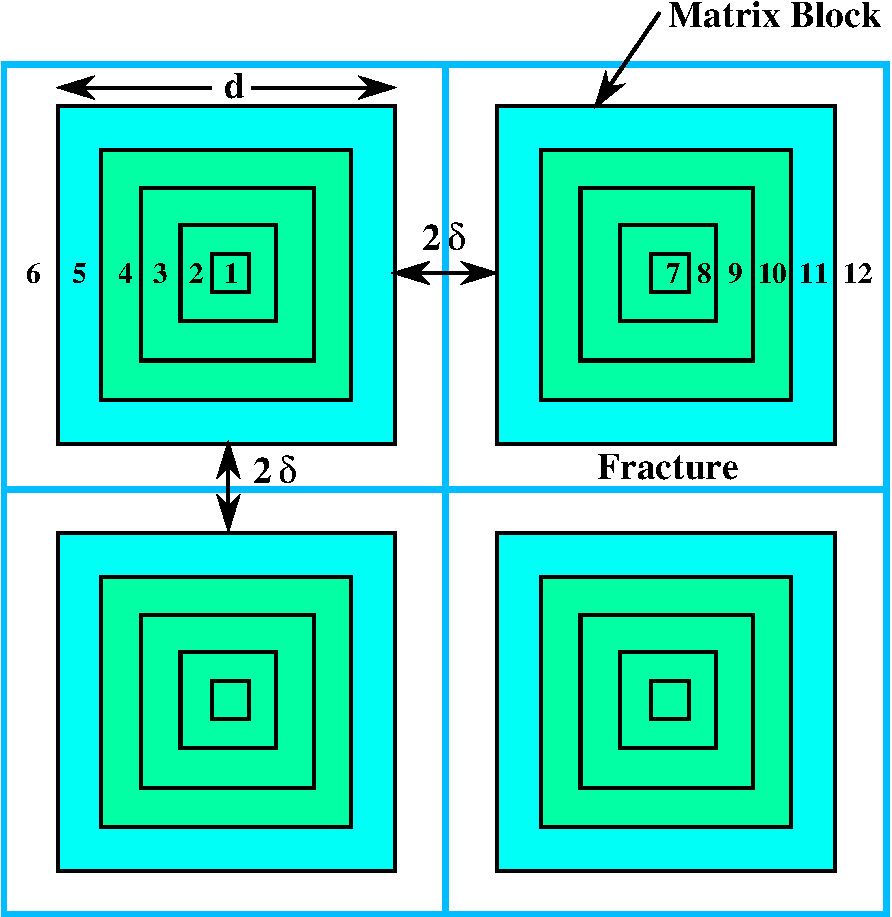
\includegraphics[scale=0.5]{./figs/mincl}
\parbox{4in}{\caption{Control volumes in DCDM multiple continuum model with fracture aperture $2\delta$ and matrix block size $d$.}\label{fminc}}
\end{figure}

Thermal conductivity at the interface between two control volumes is calculated using the harmonic average
\EQ
\kappa_{ll'} \eq \frac{\kappa_l \kappa_{l'}(d_l+d_{l'})}{d_l \kappa_{l'}+d_{l'}\kappa_l}.
\EN

The fracture volume $v_n$ is related to the REV volume $V_n$ by
\EQ
\epsilon \eq \frac{v_n}{V_n}.
\EN
According to the geometry in Figure~\ref{fminc} assuming a 3D orthogonal set of fractures,
\EQ
V_n \eq (d+2\delta)^3,
\EN
and
\EQ
v_n \eq (d+2\delta)^3 - d^3,
\EN
giving
\begin{subequations}
\BA
\epsilon &\eq 1-\frac{d^3}{(d+2\delta)^3} \eq 1-\left(\dfrac{1}{1+\dfrac{2\delta}{d}}\right)^3,\\
& ~\simeq~ \frac{6\delta}{d}.
\EA
\end{subequations}
The fracture aperture $2\delta$ is found to be in terms of $\epsilon$ and $d$
\EQ
2\delta \eq d \left(\frac{1}{(1-\epsilon)^{1/3}} -1\right).
\EN
A list of different sub-continua geometries and parameters implemented in PFLOTRAN is given in Table~\ref{tdcdmgeom}. Different independent and dependent parameters for the nested cube geometry are listed in Table~\ref{tnestedcube}.
The interfacial area $A_{nn'}^\a$ between fracture control volumes is equal to $\Delta y \Delta z$,  $\Delta z \Delta x$, $\Delta x \Delta y$ for $x$, $y$, and $z$ directions, respectively. 

In the case of nested cubes there are four possible parameters $(\epsilon, \, 2\delta, \, l_m,\, l_f)$, where $l_m$ denotes the matrix block size and $l_f$ refers to the fracture spacing, two of which are independent.

The fracture-matrix interfacial area $A_{nM}$ per unit volume is equal to
\EQ
A_{nM}^\b \eq \frac{\N_\b}{V} A_\b^0,
\EN
where the number density $\N_\b/V$ of secondary continua of type $\b$ is equal to
\EQ
\frac{\N_\b}{V} \eq \frac{1}{V} \frac{V_\b}{V_\b^0} \eq \frac{\epsilon_\b}{V_\b^0},
\EN
and $A_\b^0$ and $V_\b^0$ refer to the area and volume of each geometric type as listed in Table~\ref{tdcdm}.
\begin{table}\centering
\caption{DCDM geometric parameters.}\label{tdcdmgeom}
\vspace{3mm}
\begin{tabular}{lcc}
\toprule
Geometry & Area $A_\b^0$ & Volume $V_\b^0$\\
\midrule
Slab & $A$ & $A l$ \\
Nested Cubes & $6d^2$ & $d^3$\\
Nested Spheres & $4 \pi R^2$ & $\frac{4}{3}\pi R^3$\\
\bottomrule
\end{tabular}
\end{table}
The primary-secondary coupling term can then be written in the form
\EQ
\sum_\b\frac{\kappa_{nM}^{\a\b}}{d_n+d_{M}}\big(T_n^\a-T_{M}^\b\big) A_{nM}^\b \eq V_n
\sum_\b\frac{\epsilon_\b\kappa_{nM}^{\a\b}}{d_n+d_{M}}\big(T_n^\a-T_{M}^\b\big) \frac{A_\b^0}{V_\b^0}.
\EN

\begin{table}\centering
\caption{Independent and dependent nested cube parameters.}
\label{tnestedcube}
\vspace{3mm}
\begin{tabular}{lccc}
\toprule
\multicolumn{2}{c}{Independent} & \multicolumn{2}{c}{Dependent}\\
\midrule
$\epsilon$ & $l_f$ & $2\delta = l_f - l_m$ & $l_m = l_f(1-\epsilon)^{1/3}$\\
$\epsilon$ & $l_m$ & $2\delta = l_f - l_m$ & $l_f = l_m(1-\epsilon)^{-1/3}$\\
$2\delta$ & $l_f$ & $\epsilon = 1-(l_m/l_f)^3$ & $l_m = l_f - 2\delta$\\
$2\delta$ & $l_m$ & $\epsilon = 1-(l_m/_f)^3$ & $l_f = l_m + 2\delta$\\
$2\delta$ & $\epsilon$ & $l_m = 2\delta \Big(\dfrac{1}{(1-\epsilon)^{1/3}}-1\Big)^{-1}$ & $l_m = l-2\delta$\\
\bottomrule
\end{tabular}
\end{table}

In terms of partial differential equations the heat conservation equations may be written as
\begin{subequations}
\EQ
\frac{\p}{\p t} \epsilon \Big[\varphi \sum_\a s_\a \rho_\a U_\a + (1-\varphi) \rho_r C_r T_f\Big] + \bnabla\cdot \Big(\sum_\a \bq_\a \rho_\a H_\a -
%\epsilon
\kappa_f\bnabla T_f\Big) \eq -A_{fm} \kappa_{fm}\frac{\p T_m}{\p n},
\EN
and
\EQ
\frac{\p}{\p t} \rho_r C_r T_m + \frac{\p}{\p\xi} \Big(-\kappa_m\frac{\p T_m}{\p\xi}\Big) \eq 0,
\EN
for fracture and matrix temperatures $T_f$ and $T_m$, respectively, where $\xi$ represents the matrix coordinate assumed to be an effective 1D domain. The boundary condition 
\EQ
T_m(\xi_d,\,t\,|\,\br) \eq T_f(\br,\,t),
\EN
\end{subequations}
between fracture and matrix continua is imposed, where $\xi_d$ denotes the outer boundary of the matrix.

%The fracture thermal conductivity is defined as
%\EQ
%\kappa_f \eq \epsilon^{-1}\kappa.
%\EN

\subsection{Mode: Reactive Transport (Keyword {\tt CHEMISTRY})}\label{sec:chem}

The governing mass conservation equations for the geochemical transport mode for a multiphase system written in terms of a set of independent aqueous primary or basis species with the form
\EQ\label{rteqn}
\frac{\p}{\p t}\big(\varphi \sum_\a s_\a \Psi_j^\a\big) +
\nabla\cdot\sum_\a\bOmega_j^\a 
\eq Q_j - \sum_m\nu_{jm} I_m -\frac{\p S_j}{\p t},
\EN
and
\EQ
\frac{\p\varphi_m}{\p t} \eq \overline V_m I_m,
\EN
for minerals with molar volume $\overline V_m$, mineral reaction rate $I_m$ and mineral volume fraction $\varphi_m$ referenced to an REV. 
Sums over $\a$ in Eqn.\eqref{rteqn} are over all fluid phases in the system. The quantity $\Psi_j^\a$ denotes the total concentration of the $j$th primary species $\A_j^{\rm pri}$ in the $\a$th fluid phase defined by
\EQ
\Psi_j^\a = \delta_{l\a}^{} C_j^l + \sum_{i=1}^{N_{\rm sec}}\nu_{ji}^{\a} C_i^\a.
\EN
In this equation the subscript $l$ represents the aqueous electrolyte phase from which the primary species are chosen. The secondary species concentrations $C_i^\a$ are obtained from mass action equations corresponding to equilibrium conditions of the reactions
\EQ
\sum_j\nu_{ji}^\a\A_j^l \arrows \A_i^\a,
\EN
yielding
\EQ
C_i^\a \eq \frac{K_i^\a}{\gamma_i^\a} \prod_j \Big(\gamma_j^l C_j^l\Big)^{\nu_{ji}^\a},
\EN
with equilibrium constant $K_i^\a$, and activity coefficients $\gamma_k^\a$.
The total flux $\bOmega_j^\a$ for species-independent diffusion is given by
\EQ
\bOmega_j^\a \eq \big(\bq_\a - \varphi s_\a \bD_\a\bnabla\big)\Psi_j^\a.
\EN
The diffusion/dispersion coefficient $\bD_\a$ may be different for different phases, e.g. an aqueous electrolyte solution or gas phase, but is assumed to be species independent. Dispersivity currently must be described through a diagonal dispersion tensor. The Darcy velocity $\bq_\a$ for phase $\a$ is given by
\EQ
\bq_a \eq -\frac{kk_\a}{\mu_\a} \bnabla \big(p_\a -\rho_\a g z\big),
\EN
with bulk permeability of the porous medium $k$ and relative permeability $k_\a$, fluid viscosity $\mu_\a$, pressure $p_\a$, density $\rho_\a$, and acceleration of gravity $g$. The diffusivity/dispersivity tensor $\bD_\a$ is the sum of contributions from molecular diffusion and dispersion which for an isotropic medium has the form
\EQ
\bD_\a \eq %\varphi s 
%\Big(
\tau D_m \bI + a_T v\bI + \big(a_L-a_T\big)\frac{\bv\bv}{v},
%\Big),
\EN
with longitudinal and transverse dispersivity coefficients $a_L$, $a_T$, respectively, $\tau$ refers to tortuosity, and $D_m$ to the molecular diffusion coefficient. Currently, only longitudinal dispersion is implemented in PFLOTRAN.

The porosity may be calculated from the mineral volume fractions according to the relation
\EQ
\varphi \eq 1 - \sum_m \varphi_m. 
\EN

The temperature dependence of the diffusion coefficient is defined through the relation
\EQ
D_m(T) \eq D_m^\circ\exp\left[\frac{A_D}{R}\left(\frac{1}{T_0}-\frac{1}{T}\right)\right],
\EN
with diffusion activation energy $A_D$ in kJ/mol. The quantity $D_m^\circ$ denotes the diffusion coefficient at the reference temperature $T_0$ taken as 25\degc\ and the quantity $R$ denotes the gas constant ($8.317\times 10^{-3}$ kJ/mol/K).
The temperature $T$ is in Kelvin.

The quantity $Q_j$ denotes a source/sink term 
\EQ
Q_j \eq \sum_n\frac{q_M}{\rho}\Psi_j \delta(\br-\br_{n}),
\EN
where $q_M$ denotes a mass rate in units of kg/s, $\rho$ denotes the fluid density in kg/m$^3$, and $\br_{n}$ refers to the location of the $n$th source/sink. The quantity $S_j$ represents the sorbed concentration of the $j$th primary species considered in more detail in the next section.

Molality $m_i$ and molarity $C_i$ are related by the density of water $\rho_w$
\EQ
C_i \eq \rho_w m_i,
\EN
The activity of water is calculated from the approximate relation
\EQ
a_{\rm H_2O}^{} \eq 1 - 0.017 \sum_i m_i.
\EN

\subsubsection{Mineral Precipitation and Dissolution}

The reaction rate $I_m$ is based on transition state theory with the form
\EQ\label{Im}
I_m \eq -a_m\left(\sum_l k_{ml}(T) \P_{ml}\right) \Big(1-K_m Q_m\Big),
\EN
where the sum over $l$ represents contributions from parallel reaction mechanisms such as pH dependence etc., and where $K_m$ denotes the equilibrium constant, $a_m$ refers to the specific mineral surface area, and the ion activity product $Q_m$ is defined as
\EQ
Q_m \eq \prod_j \big(\gamma_j m_j\big)^{\nu_{jm}},
\EN
with molality $m_j$. The rate constant $k_{ml}$ is a function of temperature given by the Arrhenius relation
\EQ
k_{ml} (T) \eq k_{ml}^0 \exp\left[\frac{E_{ml}}{R}\Big(\frac{1}{T_0}-\frac{1}{T}\Big)\right],
\EN
where $k_{ml}^0$ refers to the rate constant at the reference temperature $T_0$ taken as 25\degc, with $T$ in units of Kelvin, $E_{ml}$ denotes the activation energy (kJ/mol),
and the quantity $\P_{ml}$ denotes the prefactor for the $l$th parallel reaction with the form
\EQ\label{prefactor}
\P_{ml} \eq \prod_i\dfrac{\big(\gamma_i m_i\big)^{\a_{il}^m}}{1+K_{ml}\big(\gamma_i m_i\big)^{\b_{il}^m} },
\EN
where the product index $i$ generally runs over both primary and secondary species, the quantities $\a_{il}^m$ and $\b_{il}^m$ refer to prefactor coefficients, and $K_{ml}$ is an attenuation factor.
The quantity $R$ denotes the gas constant ($8.317\times 10^{-3}$ kJ/mol/K). 

\paragraph{Rate Limiter}

A rate-limited form of the mineral kinetic rate law can be devised according to the expression
\EQ\label{ratemintran}
\widehat I_m \eq -a_m^{} \left(\sum_l \P_{ml}^{} k_{ml}^{}\right) \left[ \dfrac{1-\left(K_m Q_m\right)^{1/\sigma_m}}{1+\dfrac{k_{ml}^{}}{k_{ml}^{\rm lim}} \left(K_m Q_m\right)^{1/\sigma_m}} \right],
\EN
with rate-limiter $r_{\rm lim}$. In the limit $K_mQ_m\rightarrow\infty$, the rate becomes
\EQ
\lim_{K_m Q_m\rightarrow\infty}\widehat I_m \eq k_{ml}^{\rm lim} a_m^{}\sum_l \P_{ml}^{}.
\EN
Defining the affinity factor
\EQ
\Omega_m \eq 1-\left(K_m Q_m\right)^{1/\sigma_m},
\EN
or
\EQ
K_mQ_m \eq \Big(1-\Omega_m\Big)^{\sigma_m},
\EN
the rate may be expressed alternatively as
\EQ
\widehat I_m \eq -a_m^{} \sum_l \P_{ml}^{} k_{ml}^{} 
\dfrac{\Omega_m}{1+\dfrac{k_{ml}^{}}{k_{ml}^{\rm lim}} \big(1-\Omega_m\big)}.
\EN

\paragraph{Changes in Material Properties}

Porosity, permeability, tortuosity and mineral surface area may be updated optionally due to mineral precipitation and dissolution reactions according to the relations
\EQ\label{porosity}
\varphi \eq 1-\sum_m\varphi_m,
\EN
\EQ\label{permeability}
k \eq k_0 f(\varphi,\,\varphi_0,\,\varphi_c,\,a),
\EN
with
\BA
f &\eq \left(\frac{\varphi-\varphi_c}{\varphi_0-\varphi_c}\right)^a,\label{permf}\\
&\eq f_{\rm min} \ \ \ \text{if} \ \ \ \varphi \leq \varphi_c,\label{fmin}
\EA
\EQ\label{tortuosity}
\tau \eq \tau_0 \left(\frac{\varphi}{\varphi_0}\right)^b,
\EN
and
\EQ\label{surface_area_vf}
a_m \eq a_m^0 \left(\frac{\varphi_m}{\varphi_m^0}\right)^n  \left(\frac{1-\varphi}{1-\varphi_0}\right)^{n'},
\EN
where the super/subscript 0 denotes initial values, with a typical value for $n$ of $2/3$ reflecting the surface to volume ratio. Note that this relation only applies to primary minerals $(\varphi_m^0\ne 0)$. The quantity $\varphi_c$ refers to a critical porosity below which the permeability is assumed to be constant with scale factor $f_{\rm min}$.

In PFLOTRAN the solid is represented as an aggregate of minerals described quantitatively by specifying its porosity $\varphi$ and the volume fraction $\varphi_m$ of each primary mineral. It is not necessary  that Eqn.\eqref{porosity} relating porosity and mineral volume fractions holds. Typically, however, the solid composition is specified by giving the mass fraction $y_m$ of each of the primary minerals making up the solid phase. The volume fraction is related to mole $x_m$ and mass $y_m$ fractions by the expressions
\begin{subequations}
\BA
\varphi_m &\eq (1-\varphi) \frac{x_m \overline V_m}{\sum_{m'} x_{m'} \overline V_{m'}},\\
&\eq (1-\varphi) \frac{y_m^{} \rho_m^{-1}}{\sum_{m'} y_{m'}^{} \rho_{m'}^{-1}},
\EA
\end{subequations}
with inverse relation
\EQ
x_m \eq \frac{\varphi_m}{\overline V_m \eta_s(1-\varphi)},
\EN
and similarly for the mass fraction, where
\EQ
\rho_m^{} \eq W_m^{} \overline V_m^{-1},
\EN
and the solid molar density $\eta_s$ is given by
\EQ
\eta_s \eq \frac{1}{\sum_m x_m \overline V_m}.
\EN
In these relations $W_m$ refers to the formula weight and $\overline V_m$ the molar volume of the $m$th mineral. 
The solid molar density is related to the mass density $\rho_s$ by
\EQ
\rho_s \eq W_s \eta_s,
\EN
with the mean molecular weight $W_s$ of the solid phase equal to
\EQ
W_s \eq \sum_m x_m W_m \eq \frac{1}{\sum_m W_m^{-1} y_m^{}}.
\EN
Mass and mole fractions are related by the expression
\EQ
W_m x_m \eq W_s y_m.
\EN

\paragraph{Affinity Threshold}

An affinity threshold $f$ for precipitation may be introduced which only allows precipitation to occur if $K_m Q_m > f > 1$.

\paragraph{Surface Armoring}

Surface armoring occurs when one mineral precipitates on top of another mineral, blocking that mineral from reacting. Thus suppose mineral $\M_m$ is being replaced by the secondary mineral $\M_{m'}$. Blocking may be described phenomenologically by the surface area relation
\EQ\label{surface_armoring}
a_m(t) \eq a_m^0  \left(\frac{\varphi_m}{\varphi_m^0}\right)^n  \left(\frac{1-\varphi}{1-\varphi_0}\right)^{n'} \left(\frac{\varphi_{m'}^c - \varphi_{m'}}{\varphi_{m'}^c}\right)^{n''},
\EN
for $\varphi_{m'} < \varphi_{m'}^c$, and 
\EQ
a_m \eq 0,
\EN
if $\varphi_{m'}(t) \geq \varphi_{m'}^c$, where $\varphi_{m'}^c$ represents the critical volume fraction necessary for complete blocking of the reaction of mineral $\M_m$.

\subsubsection{Sorption}

Sorption reactions incorporated into PFLOTRAN consist of ion exchange and surface complexation reactions for both equilibrium and multirate formulations.

\paragraph{Ion Exchange}

Ion exchange reactions may be represented either in terms of bulk- or mineral-specific rock properties.  Changes in bulk sorption properties can be expected as a result of mineral reactions.  However, only the mineral-based formulation enables these effects to be captured in the model.  The bulk rock sorption site concentration $\omega_\a$, in units of moles of sites per bulk sediment volume (mol/dm$^3$), is related to the bulk cation exchange capacity $Q_\a$ (mol/kg) by the expression
\EQ
\omega_\a \eq \frac{N_{\rm site}}{V} \eq \frac{N_{\rm site}}{M_s} \frac{M_s}{V_s} \frac{V_s}{V} \eq Q_\a \rho_s (1-\phi).
\EN
The cation exchange capacity associated with the $m$th mineral is defined on a molar basis as
\EQ
\omega_m^{\rm CEC} \eq \frac{N_m}{V} \eq \frac{N_m}{M_m} \frac{M_m}{V_m} \frac{V_m}{V} \eq Q_m^{\rm CEC} \rho_m \phi_m.
\EN

In PFLOTRAN ion exchange reactions are expressed in the form
\EQ\label{ex1}
z_i \A_j + z_j X_{z_i}^\a\A_i \arrows z_j \A_i + z_i X_{z_j}^\a\A_j,
\EN
with valencies $z_j$, $z_i$ of cations $\A_j$ and $\A_i$, respectively. The reference cation is denoted by $\A_j$ and $\A_i, \,i\!\ne\! j$ represents all other cations. 
The corresponding mass action equation is given by
\EQ\label{ionexmassact}
K_{ji}^\a \eq \frac{(k_j^\a)^{z_i}}{(k_i^\a)^{z_j}} \eq \left(\frac{X_j^\a}{a_j}\right)^{z_i} \left(\frac{a_i}{X_i^\a}\right)^{z_j}.
\EN
Using the Gaines-Thomas convention, the equivalent fractions $X_k^\a$ are defined by
\EQ
X_k^\a = \frac{z_k S_k^\a}{\displaystyle\sum_l z_l S_l^\a} = \frac{z_k}{\omega_\a}S_k^\a,
\EN
with 
\EQ
\sum_k X_k^\a = 1.
\EN
The site concentration $\omega_\a$ is defined by
\EQ
\omega_\a = \sum_k z_k S_k^\a,
\EN
where $\omega_\a$ is related to the cation exchange capacity $Q_\a$ (CEC) by the expression
\EQ
\omega_\a = (1-\varphi) \rho_s \, Q_\a,
\EN
with solid density $\rho_s$ and porosity $\varphi$. 

An alternative form of reactions \ref{ex1} often found in the literature is
\EQ\label{rxn2}
\frac{1}{z_j} \A_j + \frac{1}{z_i} X_{z_i}^\a\A_i \arrows \frac{1}{z_i} \A_i + \frac{1}{z_j} X_{z_j}^\a\A_j,
\EN
obtained by dividing reaction \ref{ex1} through by the product $z_i z_j$.  In addition the reaction may be written in reverse order.
The mass action equations corresponding to reactions \ref{rxn2} have the form
\EQ
{K'}_{ji}^\a \eq \frac{({k'}_j^\a)^{1/z_j}}{({k'}_i^\a)^{1/z_i}} \eq \left(\frac{X_j^\a}{a_j}\right)^{1/z_j} \left(\frac{a_i}{X_i^\a}\right)^{1/z_i}.
\EN
The selectivity coefficients corresponding to the two forms are related by the expression
\EQ
K_{ji}^\a \eq \left({K'}_{ji}^\a\right)^{z_i z_j},
\EN
and similarly for $k_i^\a$, $k_j^\a$. When comparing with other formulations it is important that the user determine which form of the ion exchange reactions are being used and make the appropriate transformations.

For equivalent exchange $(z_j\!=\!z_i\!=\!z)$, an explicit expression exists for the sorbed concentrations given by
\EQ
S_j^\a \eq \frac{\omega_\a}{z} \frac{k_j^\a \gamma_j m_j^{}}{\displaystyle\sum_l k_l^\a \gamma_l m_l^{}},
\EN
where $m_k$ denotes the $k$th cation molality. This expression follows directly from the mass action equations and conservation of exchange sites.

In the more general case $(z_i\ne z_j)$ it is necessary to solve the nonlinear equation
\EQ
X_j^\a + \sum_{i\ne j} X_i^\a \eq 1,
\EN
for the reference cation mole fraction $X_j$. 
From the mass action equation Eqn.\eqref{ionexmassact}
it follows that
\EQ
X_i^\a\eq k_i^\a a_i\left(\frac{X_j^\a}{k_j^\a a_j}\right)^{z_i/z_j}.
\EN
Defining the function
\EQ
f(X_j^\a) \eq X_j^\a + \sum_{i\ne j}X_i^\a(X_j^\a)-1,
\EN
its derivative is given by
\EQ
\frac{df}{dX_j^\a} \eq 1 - \frac{1}{z_jX_j^\a}\sum_{i\ne j} z_i k_i^\a a_i \left(\frac{X_j^\a}{k_j^\a a_j}\right)^{z_i/z_j}.
\EN
The reference mole fraction is then obtained by Newton-Raphson iteration
\EQ
(X_j^\a)^{k+1} \eq (X_j^\a)^k -\dfrac{f[(X_j^\a)^k]}{\dfrac{df[(X_j^\a)^k]}{dX_j^\a}}.
\EN

The sorbed concentration for the $j$th cation appearing in the accumulation term is given by
\EQ
S_j^\a \eq \frac{\omega_\a}{z_j} X_j^\a,
\EN
with the derivatives for $j\ne l$
\begin{subequations}
\BA
\dfrac{\p S_j^\a}{\p m_l} &\eq -\frac{\omega_\a}{m_l} \dfrac{X_j^\a X_l^\a}{\displaystyle\sum_l z_l X_l^\a},\\
&\eq -\frac{1}{m_l} \dfrac{z_jz_lS_j^\a S_l^\a}{\displaystyle\sum_l z_l^2 S_l^\a},
\EA
\end{subequations}
and for $j=l$
\begin{subequations}
\BA
\dfrac{\p S_j^\a}{\p m_j} &\eq \frac{\omega_\a X_j^\a}{z_j m_j} \left(1-\dfrac{z_j X_j^\a}{\displaystyle\sum_{l} z_{l} X_{l}^\a}\right),\\
&\eq \frac{S_j^\a}{m_j} \left(1-\dfrac{z_j^2 S_j^\a}{\displaystyle\sum_{l} z_{l}^2 S_{l}^\a}\right).
\EA
\end{subequations}

\paragraph{Surface Complexation}

Surface complexation reactions are assumed to have the form
\EQ\label{srfrxn}
\nu_\a >\!\!\chi_\a + \sum_j\nu_{ji} \A_j \arrows \!>\!\! \mcS_{i\a},
\EN
for the $i$th surface complex $>\!\!\mcS_{i\a}$ on site $\a$ and empty site $>\!\!\chi_\a$.
As follows from the corresponding mass action equation the equilibrium sorption concentration $S_{i\a}^{\rm eq}$ is given by
\EQ
S_{i\a}^{\rm eq}\eq \frac{\omega_\a K_i Q_i}{1+\sum_l K_lQ_l},
\EN
and the empty site concentration by
\EQ
S_\a^{\rm eq}\eq\frac{\omega_\a}{1+\sum_l K_lQ_l},
\EN
where the ion activity product $Q_i$ is defined by
\EQ
Q_i\eq\prod_j\big(\gamma_jC_j\big)^{\nu_{ji}}.
\EN
The site concentration $\omega_\a$ satisfies the relation
\EQ\label{totsite}
\omega_\a \eq S_\a + \sum_i S_{i\a},
\EN
and is constant.
The equilibrium sorbed concentration $S_{j\a}^{\rm eq}$ is defined as
\EQ\label{qeq}
S_{j\a}^{\rm eq} \eq \sum_i \nu_{ji}^{} S_{i\a}^{\rm eq}\eq \frac{\omega_\a}{1+\sum_l K_lQ_l} \sum_i \nu_{ji}K_i Q_i.
\EN

\paragraph{Multirate Sorption}

In the multirate model the rates of sorption reactions are described through a kinetic relation given by
\EQ\label{sorbed}
\frac{\p S_{i\a}}{\p t} \eq k_\a^{} \big(S_{i\a}^{\rm eq}-S_{i\a}\big),
\EN
for surface complexes, and
\BA\label{fsite}
\frac{\p S_{\a}}{\p t} &\eq -\sum_i k_\a^{} \big(S_{i\a}^{\rm eq}-S_{i\a}\big),\\
&\eq k_\a\big(S_\a^{\rm eq}-S_{\a}\big),
\EA
for empty sites, where $S_\a^{\rm eq}$ denotes the equilibrium sorbed concentration. For simplicity, in what follows it is assumed that $\nu_\a\!=\!1$. 
With each site $\a$ is associated a rate constant $k_\a$ and site concentration $\omega_\a$. These quantities are defined through a given distribution of sites $\wp(\a)$, such that
\EQ
\int_0^\infty \wp(k_\a)dk_\a \eq 1.
\EN
The fraction of sites $f_\a$ belonging to site $\a$ is determined from the relation
\EQ
f_\a \eq \int_{k_\a-\Delta k_\a/2}^{k_\a+\Delta k_\a/2} \wp(k_\a)dk_\a \simeq \wp(k_\a)\Delta k_\a,
\EN
with the property that
\EQ
\sum_\a f_\a =1.
\EN
Given that the total site concentration is $\omega$, then the site concentration $\omega_\a$ associated with site $\a$ is equal to
\EQ
\omega_\a \eq f_\a \omega.
\EN

An alternative form of these equations is obtained by introducing the total sorbed concentration for the $j$th primary species for each site defined as
\EQ
S_{j\a}\eq\sum_i \nu_{ji}S_{i\a}.
\EN
Then the transport equations become
\EQ\label{totj}
\frac{\p}{\p t}\left(\varphi \Psi_j + \sum_{\a}S_{j\a}\right) + \bnabla\cdot\bOmega_j \eq  - \sum_m\nu_{jm}I_m.
\EN
The total sorbed concentrations are obtained from the equations
\EQ\label{sja}
\frac{\p S_{j\a}}{\p t} \eq k_\a^{} \big(S_{j\a}^{\rm eq}-S_{j\a}\big).
\EN

\subsubsection{Sorption Isotherm}

A sorption isotherm $S_j$ may be specified for any primary species $\A_j$. 
The following transport equation is solved 
\EQ
\frac{\p}{\p t} \varphi s C_j + \bnabla\cdot\bF_j \eq -\frac{\p S_j}{\p t},
\EN
with $C_j \eq \rho_w m_j$ and $\rho_w$ refers to the density of pure water.
Three distinct models are available for the sorption isotherm $S_j$:
\begin{itemize}
\item linear $K_D$ model
\EQ\label{linkd}
S_j \eq K_j^D \gamma_j m_j,
\EN
with activity coefficient $\gamma_j$ and molality $m_j$,
\item Langmuir isotherm:
\EQ\label{Langmuir}
S_j \eq \frac{K_j^L b_j^L \gamma_j m_j}{(1+K_j^L \gamma_j m_j)},
\EN
with Langmuir coefficients $K_j^L$ and $b_j^L$, and
\item Freundlich isotherm:
\EQ\label{Freundlich}
S_j \eq K_j^F \big(\gamma_j m_j\big)^{(1/n_j^F)},
\EN
with coefficients $K_j^F$ and $n_j^F$.
\end{itemize}
The linear $K_D$ model results in the retardation factor $\R_j$ given by
\EQ
\R_j \eq 1 + \frac{\gamma_j K_j^D}{\varphi s \rho_w}.
\EN
In terms of the retardation the transport equation becomes
\EQ
\frac{\p}{\p t} \big(\R_j\varphi s \rho_w m_j\big) + \bnabla\cdot\bF_j \eq 0.
\EN

\subsubsection{Colloid-Facilitated Transport}

Colloid-facilitated transport is implemented into PFLOTRAN based on surface complexation reactions. Competition between mobile and immobile colloids and stationary mineral surfaces is taken into account. Colloid filtration processes are not currently implemented into PFLOTRAN. 
A colloid is treated as a solid particle suspended in solution or attached to a mineral surface. Colloids may be generated through nucleation of minerals in solution, although this effect is not included currently in the code.

Three separate reactions may take place involving competition between mobile and immobile colloids and mineral surfaces
\BA
>\!X_k^\m + \sum_j\nu_{jk}\A_j &\arrows >\!S_k^\m,\\
>\!X_k^\im + \sum_j\nu_{jk}\A_j &\arrows >\!S_k^\im,\\
>\!X_k^s + \sum_j\nu_{jk}\A_j &\arrows >\!S_k^s,
\EA
with corresponding reaction rates $I_k^\m$, $I_k^\im$, and $I_k^s$, where the superscripts $s$, $m$, and $im$ denote mineral surfaces, and mobile and immobile colloids, respectively. In addition, reaction with minerals $\M_s$ may occur according to the reaction
\EQ
\sum_j\nu_{js}\A_j \arrows \M_s.
\EN
The transport equations for primary species, mobile and immobile colloids, read
\BA
\frac{\p}{\p t} \varphi s_l \Psi_j^l + \bnabla\cdot\bOmega_j^l &\eq -\sum_k\nu_{jk}\big(I_k^\m + I_k^\im + \sum_s I_k^s\big) - \sum_s \nu_{js} I_s,\label{rateform}\\
\frac{\p}{\p t} \varphi s_l S_k^\m + \bnabla\cdot\bq_c S_k^\m & \eq I_k^\m,\label{mobile}\\
\frac{\p}{\p t} S_k^\im & \eq I_k^\im,\label{immobile}\\
\frac{\p}{\p t} S_k^s & \eq I_k^s,\label{solid}
\EA
where $\bq_c$ denotes the colloid Darcy velocity which may be greater than the fluid velocity $\bq$.
For conditions of local equilibrium the sorption reaction rates may be eliminated and replaced by algebraic sorption isotherms to yield
\EQ\label{eqform}
\frac{\p}{\p t}\Big[ \varphi s_l \Psi_j^l + \sum_k \nu_{jk} \big(\varphi s_l S_k^\m + S_k^\im + \sum_s S_k^s\big) \Big] + \bnabla\cdot\Big(\bOmega_j^l + \bq_c \sum_k \nu_{jk} S_k^\m\Big) \eq - \sum_s \nu_{js} I_s.
\EN

In the kinetic case either form of the primary species transport equations given by Eqn.\eqref{rateform} or \eqref{eqform} can be used provided it is coupled with the appropriate kinetic equations Eqns.\eqref{mobile}--\eqref{solid}. The mobile case leads to additional equations that must be solved simultaneously with the primary species equations. A typical expression for $I_k^m$ might be
\EQ
I_k^m \eq k_k\big(S_k^m - S_{km}^{\rm eq}\big),
\EN
with rate constant $k_k$ and where $S_{km}^{\rm eq}$ is a known function of the solute concentrations. In this case, Eqn.\eqref{mobile} must be added to the primary species transport equations. Further reduction of the transport equations for the case where a flux term is present in the kinetic equation is not possible in general for complex flux terms.

\subsection{Tracer Mean Age}

PFLOTRAN implements the Eulerian formulation of solute age for a nonreactive tracer following Goode (1996). PFLOTRAN solves the advection-diffusion/dispersion equation for the mean age given by
\EQ
\frac{\p}{\p t} \varphi s AC + \bnabla\cdot\Big(\bq AC - \varphi s D \bnabla (AC)\Big) \eq \varphi s C,
\EN
where $A$ denotes the mean age of the tracer with concentration $C$. Other quantities appearing in the age equation are identical to the tracer transport equation for a partially saturated porous medium with saturation state $s$. The age and tracer transport equations are solved simultaneously for the age-concentration $\alpha = A C$ and tracer concentration $C$. The age-concentration $\a$ satisfies the usual advection-diffusion-dispersion equation with a source term on the right-hand side.

The mean tracer is calculated in PFLOTRAN by adding the species {\tt Tracer\_Age} together with {\tt Tracer} to the list of primary species
%\newpage
\begin{verbatim}
  PRIMARY_SPECIES
    Tracer
    Tracer_Age
  /
\end{verbatim}
including sorption through a constant $K_d$ model if desired
\begin{verbatim}
  SORPTION
    ISOTHERM_REACTIONS
      Tracer
        TYPE LINEAR 
        DISTRIBUTION_COEFFICIENT 500. ! kg water/m^3 bulk
      /
      Tracer_Age
        TYPE LINEAR 
        DISTRIBUTION_COEFFICIENT 500. ! kg water/m^3 bulk
      /
    /
  /
\end{verbatim}
and specifying these species in the initial and boundary {\tt CONSTRAINT} condition as e.g.:
\begin{verbatim}
CONSTRAINT initial
  CONCENTRATIONS
    Tracer     1.e-8        F
    Tracer_Age 1.e-16       F
  /
/
\end{verbatim}
Output is given in terms of $\alpha$ and $C$ from which the mean age $A$ can be obtained as $A\eq\alpha/C$. 

\subsection{Thermodynamic Database}
\label{thermo:database}

PFLOTRAN reads thermodynamic data from a database that may be customized by the user. Reactions included in the database consist of aqueous complexation, mineral precipitation and dissolution, gaseous reactions, and surface complexation. Ion exchange reactions and their selectivity coefficients are entered directly from the input file. 
A standard database supplied with the code is referred to as {\tt hanford.dat} and is found in the {\tt ./database} directory in the PFLOTRAN mercurial repository. This database is an ascii text file that can be edited by any editor and is equivalent to the EQ3/6 database:
\begin{verbatim}
data0.com.V8.R6
CII: GEMBOCHS.V2-EQ8-data0.com.V8.R6
THERMODYNAMIC DATABASE
generated by GEMBOCHS.V2-Jewel.src.R5 03-dec-1996 14:19:25
\end{verbatim}
The database provides equilibrium constants in the form of log $K$ values at a specified set of temperatures listed in the top line of the database. A least squares fit is used to interpolate the log $K$ values between the database temperatures using a Maier-Kelly expansion of the form
\EQ\label{mk}
\log K \eq c_{-1} \ln T + c_0 + c_1 T + \frac{c_2}{T} + \frac{c_3}{T^2},
\EN
with fit coefficients $c_i$. 
The thermodynamic database stores all chemical reaction properties (equilibrium constant $\log K_r$, reaction stoichiometry $\nu_{ir}$, species valence $z_i$, Debye parameter $a_i$, mineral molar volume $\overline V_m$, and formula weight $w_i$) used in PFLOTRAN. The database is divided into 5 blocks as listed in Table~\ref{tdatabase}, consisting of
database primary species, aqueous complex reactions, gaseous reactions, mineral reactions, and surface complexation reactions. 
Each block is terminated by a line beginning with {\tt 'null'}. 
The quantity $N_{\rm temp}$ refers to the number of temperatures at which log $K$ values are stored in the database.
In the {\tt hanford.dat} database $N_{\rm temp}=8$ with equilibrium constants stored at the temperatures: 0, 25, 60, 100, 150, 200, 250, and 300\degc. The pressure is assumed to lie along the saturation curve of pure water for temperatures above 25\degc\ and is equal to 1 bar at lower temperatures.
Reactions in the database are assumed to be written in the canonical form
\EQ
\A_r \arrows \sum_{i=1}^{\rm nspec} \nu_{ir}\A_i,
\EN
for species $\A_r$, where {\tt nspec} refers to the number of aqueous or gaseous species $\A_i$ on the right-hand side of the reaction. 
Redox reactions in the standard database {\tt hanford.dat} are usually written in terms of O$_{2(g)}$.
Complexation reactions involving redox sensitive species are written in such a manner as to preserve the redox state.


\begin{table}[h]\centering
\caption{Format of thermodynamic database.}\label{tdatabase}
\vspace{3mm}
%\footnotesize
\begin{tabular}{ll}
\hline
Primary Species: & name, $a_0$, $z$, $w$\\
Secondary Species: & name, nspec, ($\nu$(n), name($n$), $n$=1, nspec), log$K$(1:$N_{\rm temp}$), $a_0$, $z$, $w$\\
Gaseous Species: & name, $\overline V$, nspec, ($\nu$(n), name($n$), $n$=1, nspec), log$K$(1:$N_{\rm temp}$), $w$ \\
Minerals: & name, $\overline V$, nspec, ($\nu$(n), name($n$), $n$=1, nspec), log$K$(1:$N_{\rm temp}$), $w$\\
Surface Complexes: & $>$name, nspec, $\nu$, $>$site, 
($\nu$(n), name($n$), $n$=1, nspec-1), \\
&\hspace{3in} log$K$(1:$N_{\rm temp}$), $z$, $w$\\
\hline
\end{tabular}
\end{table}

\subsection{Eh, pe}

Output for Eh and pe is calculated from the half-cell reaction
\EQ\label{redox}
\rm 2 \, H_2O - 4 \, H^+ - 4\,e^- \arrows \rm O_2,
\EN
with the corresponding equilibrium constant fit to the Maier-Kelly expansion Eqn.\eqref{mk}. The fit coefficients are listed in Table~\ref{tmkfit}.

\begin{table}[H]\centering
\caption{Fit coefficients for log $K$ of reaction \ref{redox}.}
\label{tmkfit}
\vspace{3mm}
\begin{tabular}{lr}
\toprule
$c_{-1}$ & 6.745529048\\
$c_0$ & $-$48.295936593\\
$c_1$ & $-$0.000557816\\
$c_2$ & 27780.749538022\\
$c_3$ & 4027.337694858\\
\bottomrule
\end{tabular}
\end{table}

\section{Appendix: Method of Solution}

\setcounter{equation}{0}

The flow and heat equations (Modes: RICHARDS, MPHASE, FLASH2, THC, \ldots) are solved using a fully implicit backward Euler approach based on Newton-Krylov iteration.
Both fully implicit backward Euler and operator splitting solution methods are supported for reactive transport.

\subsection{Fully Implicit}

In a fully implicit formulation the nonlinear equations for the residual function $\bR$ given by
\EQ
\bR(\bx) \eq \bzero,
\EN
are solved using an iterative solver based on the Newton-Raphson equations
\EQ
\bJ^{(i)} \delta\bx^{(i+1)} \eq -\bR^{(i)},
\EN
at the $i$th iteration. Iteration stops when
\EQ
\left|\bR^{(i+1)}\right| < \epsilon,
\EN
or if
\EQ
\big|\delta\bx^{(i+1)}\big| < \delta.
\EN
However, the latter criteria does not necessarily guarantee that the residual equations are satisfied.
The solution is updated from the relation
\EQ
\bx^{(i+1)} \eq \bx^{(i)} + \delta\bx^{(i+1)}.
\EN
For the logarithm of the concentration with $\bx=\ln\by$,
the solution is updated according to the equation
\EQ
\by^{(i+1)} \eq \by^{(i)} {\rm e}^{\delta\ln\by^{(i+1)}}.
\EN

\subsubsection{Multirate Sorption}

The residual function incorporating the multirate sorption model can be further simplified by solving analytically the finite difference form of kinetic sorption equations. This is possible when these equations are linear in the sorbed concentration $S_{j\a}$ and because they do not contain a flux term. Thus discretizing Eqn.\eqref{sja} in time using the fully implicit backward Euler method gives
\EQ
\frac{S_{j\a}^{t+\Delta t}-S_{j\a}^t}{\Delta t} \eq k_\a \big(f_\a S_{j\a}^{\rm eq} - S_{j\a}^{t+\Delta t}\big).
\EN
Solving for $S_{j\a}^{t+\Delta t}$ yields
\EQ\label{sjadt}
S_{j\a}^{t+\Delta t} \eq \frac{S_{j\a}^t + k_\a \Delta t f_\a S_j^{\rm eq}}{1+k_\a\Delta t}.
\EN
From this expression the reaction rate can be calculated as
\EQ
\frac{S_{j\a}^{t+\Delta t}-S_{j\a}^t}{\Delta t} \eq \frac{k_\a}{1+k_\a\Delta t} \big(f_\a S_{j\a}^{\rm eq} - S_{j\a}^t\big).
\EN
The right-hand side of this equation is a known function of the solute concentration and thus by substituting into Eqn.\eqref{totj} eliminates the appearance of the unknown sorbed concentration. Once the transport equations are solved over a time step, the sorbed concentrations can be computed from Eqn.\eqref{sjadt}.

\subsection{Operator Splitting}

Operator splitting involves splitting the reactive transport equations into a nonreactive part and a part incorporating reactions. This is accomplished by writing Eqns.\eqref{rteqn} as the two coupled equations
\EQ
\frac{\p}{\p t}\big(\varphi \sum_\a s_\a \Psi_j^\a\big) +
\nabla\cdot\sum_\a\big(\bq_\a - \varphi s_\a \bD_\a\bnabla\big)\Psi_j^\a \eq Q_j,
\EN
and
\EQ
\frac{d}{d t}\big(\varphi \sum_\a s_\a \Psi_j^\a\big) \eq - \sum_m\nu_{jm} I_m -\frac{\p S_j}{\p t},
\EN
The first set of equations are linear in $\Psi_j$ (for species-independent diffusion coeffients) and solved over over a time step $\Delta t$ resulting in $\Psi_j^*$. The result for $\Psi_j^*$ is inverted to give the concentrations $C_j^*$ by solving the equations
\EQ
\Psi_j^* \eq C_j^* + \sum_i \nu_{ji} C_i^*,
\EN
where the secondary species concentrations $C_i^*$ are nonlinear functions of the primary species concentrations $C_j^*$. With this result the second set of equations are solved implicitly for $C_j$ at $t+\Delta t$ using $\Psi_j^*$ for the starting value at time $t$.

\subsubsection{Constant $K_d$}

As a simple example of operator splitting consider a single component system with retardation described by a constant $K_d$. According to this model the sorbed concentration $S$ is related to the aqueous concentration by the linear equation
\EQ\label{skd}
S \eq K_d C.
\EN
The governing equation is given by
\EQ
\frac{\p}{\p t} \varphi C + \bnabla\cdot\big(\bq C -\varphi D \bnabla C\big) \eq -\frac{\p S}{\p t}.
\EN
If $C(x,\,t;\, \bq,\,D)$ is the solution to the case with no retardation (i.e. $K_d=0$), then $C(x,\,t;\, \bq/R,\,D/R)$ is the solution with retardation $(K_d>0)$,
with
\EQ
R = 1+\frac{1}{\varphi}K_d.
\EN
Thus propagation of a front is retarded by the retardation factor $R$.

In operator splitting form this equation becomes
\EQ
\frac{\p}{\p t} \varphi C + \bnabla\cdot\big(\bq C -\varphi D \bnabla C\big) \eq 0,
\EN
and
\EQ
\frac{d}{d t} \varphi C \eq -\frac{d S}{d t}.
\EN
The solution to the latter equation is given by
\EQ
\varphi C^{t+\Delta t} - \varphi C^* \eq -\big(S^{t+\Delta t} - S^t\big),
\EN
where $C^*$ is the solution to the nonreactive transport equation. Using Eqn.\eqref{skd}, this result can be written as
\EQ
C^{t+\Delta t} \eq \frac{1}{R} C^* + \left(1-\frac{1}{R}\right) C^t.
\EN
Thus for $R=1$, $C^{t+\Delta t}=C^*$ and the solution advances unretarded. As $R\rightarrow\infty$, $C^{t+\Delta t} \rightarrow C^t$ and the front is fully retarded.

